%%=============================================================================
%% Inleiding
%%=============================================================================

\chapter{\IfLanguageName{dutch}{Inleiding}{Introduction}}%
\label{ch:inleiding}
Cyberbeveiliging speelt een cruciale rol binnen de bescherming van gevoelige informatie. Het is dan ook essentieel dat organisaties 
effectieve beveiligingstools implementeren om hun webomgevingen te beschermen. Penetratietesten of pentests, zijn  
methodieken om de beveiliging van webapplicaties te beoordelen door ze bloot te stellen aan gesimuleerde 
cyberaanvallen die zich focussen op het onthullen van kwetsbaarheden. Dit onderzoek gaat dieper in op de kwetsbaarheden van deze omgevingen. Het doel is om te bepalen welke tools 
het meest effectief zijn in specifieke situaties en hoe beveiligingsstrategieën aangepast kunnen worden om optimale 
bescherming te bieden.


\section{\IfLanguageName{dutch}{Probleemstelling}{Problem Statement}}%
\label{sec:probleemstelling}

\begin{figure}
  \centering
  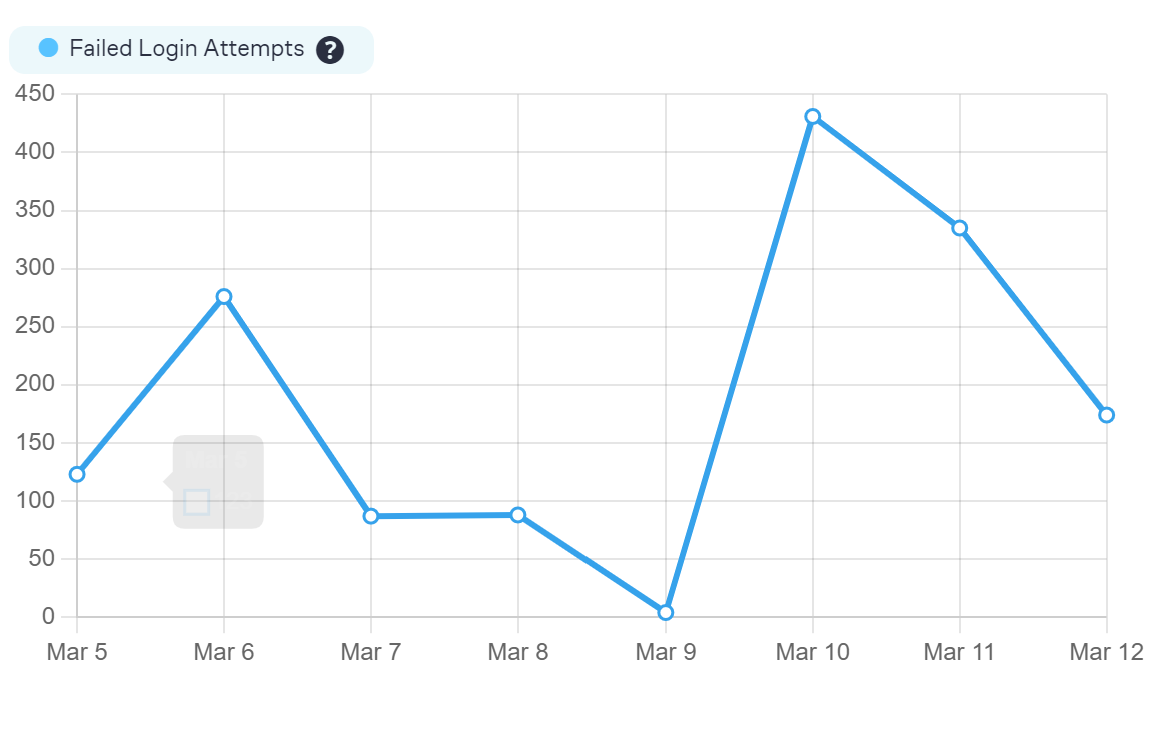
\includegraphics[height=0.3\textheight]{failed_login_attemps_24flow.png}
  \caption[aantal foutieve logins op de wordpress website van 24Flow per dag ]{aantal foutieve logins op de wordpress website van 24Flow per dag }
\end{figure}
Kleine tot middelgrote IT-servicebedrijven, zoals Sinergio (promotor van dit eindwerk) en 24Flow (stageplaats), worden net 
als elk ander bedrijf dagelijks geconfronteerd met de uitdaging om hun 
webapplicaties alsmaar beter te beschermen tegen cyberaanvallen. Deze bedrijven maken vaak gebruik van populaire webontwikkelingsplatformen 
zoals het CMS WordPress of het ontwikkelingsframework Laravel, die elk op zich unieke en specifieke beveiligingsrisico's en 
kwetsbaarheden kennen. De bescherming van deze platformen wordt dan toevertrouwd aan de implementatie van beveiligingsplugins 
en -tools, waarvan de effectiviteit varieert.

Deze bachelorproef focust zich voornamelijk op het onderzoek naar de effectiviteit van een aantal gangbare penetratietesttools  
bij het identificeren van kwetsbaarheden binnen drie specifieke webomgevingen: een WordPress applicatie zonder beveiligingsplugins,
een WordPress applicatie met beveiligingsplugins en een afgewerkte Laravel applicatie. Het doel van dit onderzoek is tweeledig. 
Ten eerste, het vaststellen welke penetratietesttool(s) het meest functioneel zijn aan de hand van objectieve criteria binnen het kader van deze webomgevingen. Ten tweede, 
een analyse maken van de beveiligingsrisico's geassocieerd met elk van de te onderzoeken omgevingen om de vraag te beantwoorden hoe 
veilig of onveilig deze wel zijn.

De directe doelgroep voor deze bachelorproef is het bedrijf Sinergio, een kleinere IT-serviceprovider die regelmatig 
werkt met WordPress en Laravel bij het ontwikkelen van websites of webapplicaties voor hun klanten. De resultaten van dit 
onderzoek biedt Sinergio dan ook waardevolle inzichten in de meest doeltreffende manieren om hun webontwikkelingsprojecten beter 
te beveiligen en geeft hun een idee hoe belangrijk het is om beveiligingsplugins te integreren binnen wordpress-applicaties. 
Dit stelt hen bovendien in staat om onderbouwde beslissingen te nemen over het gebruik van 
beveiligingsstrategieën en -tools. Sinergio zal desgevallend kunnen achterhalen welke pentesting tool het interessantst is 
binnen hun specifieke omgevingen en zal hierdoor in de toekomst dit aspect minder zelf moeten onderzoeken.
Bovendien draagt dit onderzoek bij aan een bredere kennisbasis over webapplicatiebeveiliging, 
wat van belang kan zijn voor andere kleine tot middelgrote IT-bedrijven die vergelijkbare technologieën gebruiken.

\section{\IfLanguageName{dutch}{Onderzoeksvraag}{Research question}}%
\label{sec:onderzoeksvraag}
De onderzoeksvraag wordt opgesplitst in twee luiken.
\begin{enumerate}
  \item Welke penetratietesttool(s) zijn volgens de vooraf bepaalde criteria het meest effectief/efficiënt in het identificeren van kwetsbaarheden in de drie specifieke webomgevingen?
  \item Welke specifieke kwetsbaarheden detecteren de penetratietesttools in een WordPress-omgeving zonder beveiligingsplugins en hoe verschilt dit van de omgevingen met beveiligingsplugins en de Laravel-applicatie? 
\end{enumerate}
Deze onderzoeksvragen vormen een duidelijke basis om de werking van de verschillende penetratietesttools te kunnen evalueren 
en om de impact op de geteste webomgevingen op een gestrucureerde manier te kunnen vergelijken. Door de prestaties van de 
tools te beoordelen op vlak van efficiëntie, functionaliteit, kostprijzen, ondersteuning van de community en gebruiksgemak, 
kan dit onderzoek waardevolle inzichten bieden.

\section{\IfLanguageName{dutch}{Onderzoeksdoelstelling}{Research objective}}%
\label{sec:onderzoeksdoelstelling}
De doelstelling van deze paper is het uitvoeren van een vergelijkende studie, die de effectiviteit en andere aspecten uit bovenstaand hoofdstuk 
test van verschillende penetratietesttools bij het identificeren van kwetsbaarheden in verschillende webomgevingen.
Het beoogde resultaat is een verslag met gedetailleerde aanbevelingen over de meest aangewezen voor de drie geteste 
omgevingen. Het succes werd gemeten aan de hand van de volledigheid van de verzamelde data, de analytische diepgang van de bevindingen 
en de duidelijkheid van de vergelijkende analyse tussen de tools en omgevingen. Dit verslag kan op die manier interessante inzichten bieden die 
bijdragen aan betere beveiligingsstrategieën en -implementaties in webontwikkelingsprojecten.
\section{\IfLanguageName{dutch}{Opzet van deze bachelorproef}{Structure of this bachelor thesis}}%
\label{sec:opzet-bachelorproef}

% Het is gebruikelijk aan het einde van de inleiding een overzicht te
% geven van de opbouw van de rest van de tekst. Deze sectie bevat al een aanzet
% die je kan aanvullen/aanpassen in functie van je eigen tekst.

In het verdere verloop van deze bacheloorproef komen onderstaande hoofdstukken aan bod.

Hoofdstuk~\ref{ch:stand-van-zaken} geeft een overzicht van de stand van zaken binnen het onderzoeksdomein, op basis van een literatuurstudie.

Hoofdstuk~\ref{ch:methodologie} geeft toelichting omtrent de methodologie en de gebruikte onderzoekstechnieken die een antwoord kunnen formuleren op de onderzoeksvragen.

% TODO: Vul hier aan voor je eigen hoofstukken, één of twee zinnen per hoofdstuk
Hoofdstuk~\ref{ch:resultaten} bevat de resultaten van het onderzoek.

Hoofdstuk~\ref{ch:conclusie} bevat de conclusies en hier wordt tevens een antwoord geformuleerd op de onderzoeksvragen. Daarbij wordt overigens ook een aanzet gegeven voor toekomstig onderzoek binnen dit domein.